\section{Methodology}
In robotic action prediction, most visual tokens remain static across frames except for key regions like the manipulator or target object. While this temporal redundancy enables token reuse, reusing all static tokens can harm accuracy when task-relevant regions subtly change. To address this, we propose a method that identifies visually static tokens and filters out semantically important ones based on attention scores from the VLA decoder. By avoiding redundant computation of unchanged static tokens between adjacent frames, our approach directly alleviates the computation bottleneck of language decoder in VLA models while preserving the accuracy of action prediction.

\subsection{KV Cache for VLA Token Reusing}
\label{sec:preliminary}
Key-Value (KV) caching is a widely adopted technique in large-scale autoregressive models to reduce both computation and memory footprint during decoding. Initially proposed in the Transformer architecture~\cite{vaswani2017attention}, KV caching enables the model to reuse previously computed key ($\mathbf{K}$) and value ($\mathbf{V}$) vectors for each token, thereby avoiding redundant computation across decoding steps. Concretely, given a sequence of input tokens $\mathbf{X}$, the self-attention mechanism computes:
\begin{equation}
\mathbf{Q} = \mathbf{X} W_Q, \quad \mathbf{K} = \mathbf{X} W_K, \quad \mathbf{V} = \mathbf{X} W_V,
\end{equation}
\begin{equation}
\mathrm{Attn}(\mathbf{Q}, \mathbf{K}, \mathbf{V}) =
\mathrm{Softmax}\left(\frac{\mathbf{Q} \mathbf{K}^\top}{\sqrt{d}}\right) \mathbf{V}.
\end{equation}

During decoding, each new token’s $\mathbf{k}_{\text{new}}$ and $\mathbf{v}_{\text{new}}$ are appended to the $i$-th cache:
\begin{equation}
\mathbf{K}_i = \mathrm{Concat}(\mathbf{K}_{i-1}, \mathbf{k}_{\text{new}}), \quad
\mathbf{V}_i = \mathrm{Concat}(\mathbf{V}_{i-1}, \mathbf{v}_{\text{new}}).
\end{equation}

While KV caching is effective for language decoding within a single query in vision-language models, this technique does not address redundancy in the visual stream, especially in Vision-Language-Action (VLA) models. In robotic manipulation, consecutive visual inputs often share large overlapping content, yet VLA models typically discard visual encodings after each step and recompute them from scratch. This is both wasteful and suboptimal for real-time control.

This inefficiency motivates a key question:  \textit{can we selectively reuse static visual tokens across time with temporal KV Caching in VLA models?} This idea forms the basis of our proposed \textbf{VLA-Cache}. In the following sections, we introduce its core mechanisms: static token selection, task-relevance filtering, and layer-adaptive reuse to accelerate VLA inference while preserving action accuracy.

\begin{figure*}[!t]
\centering
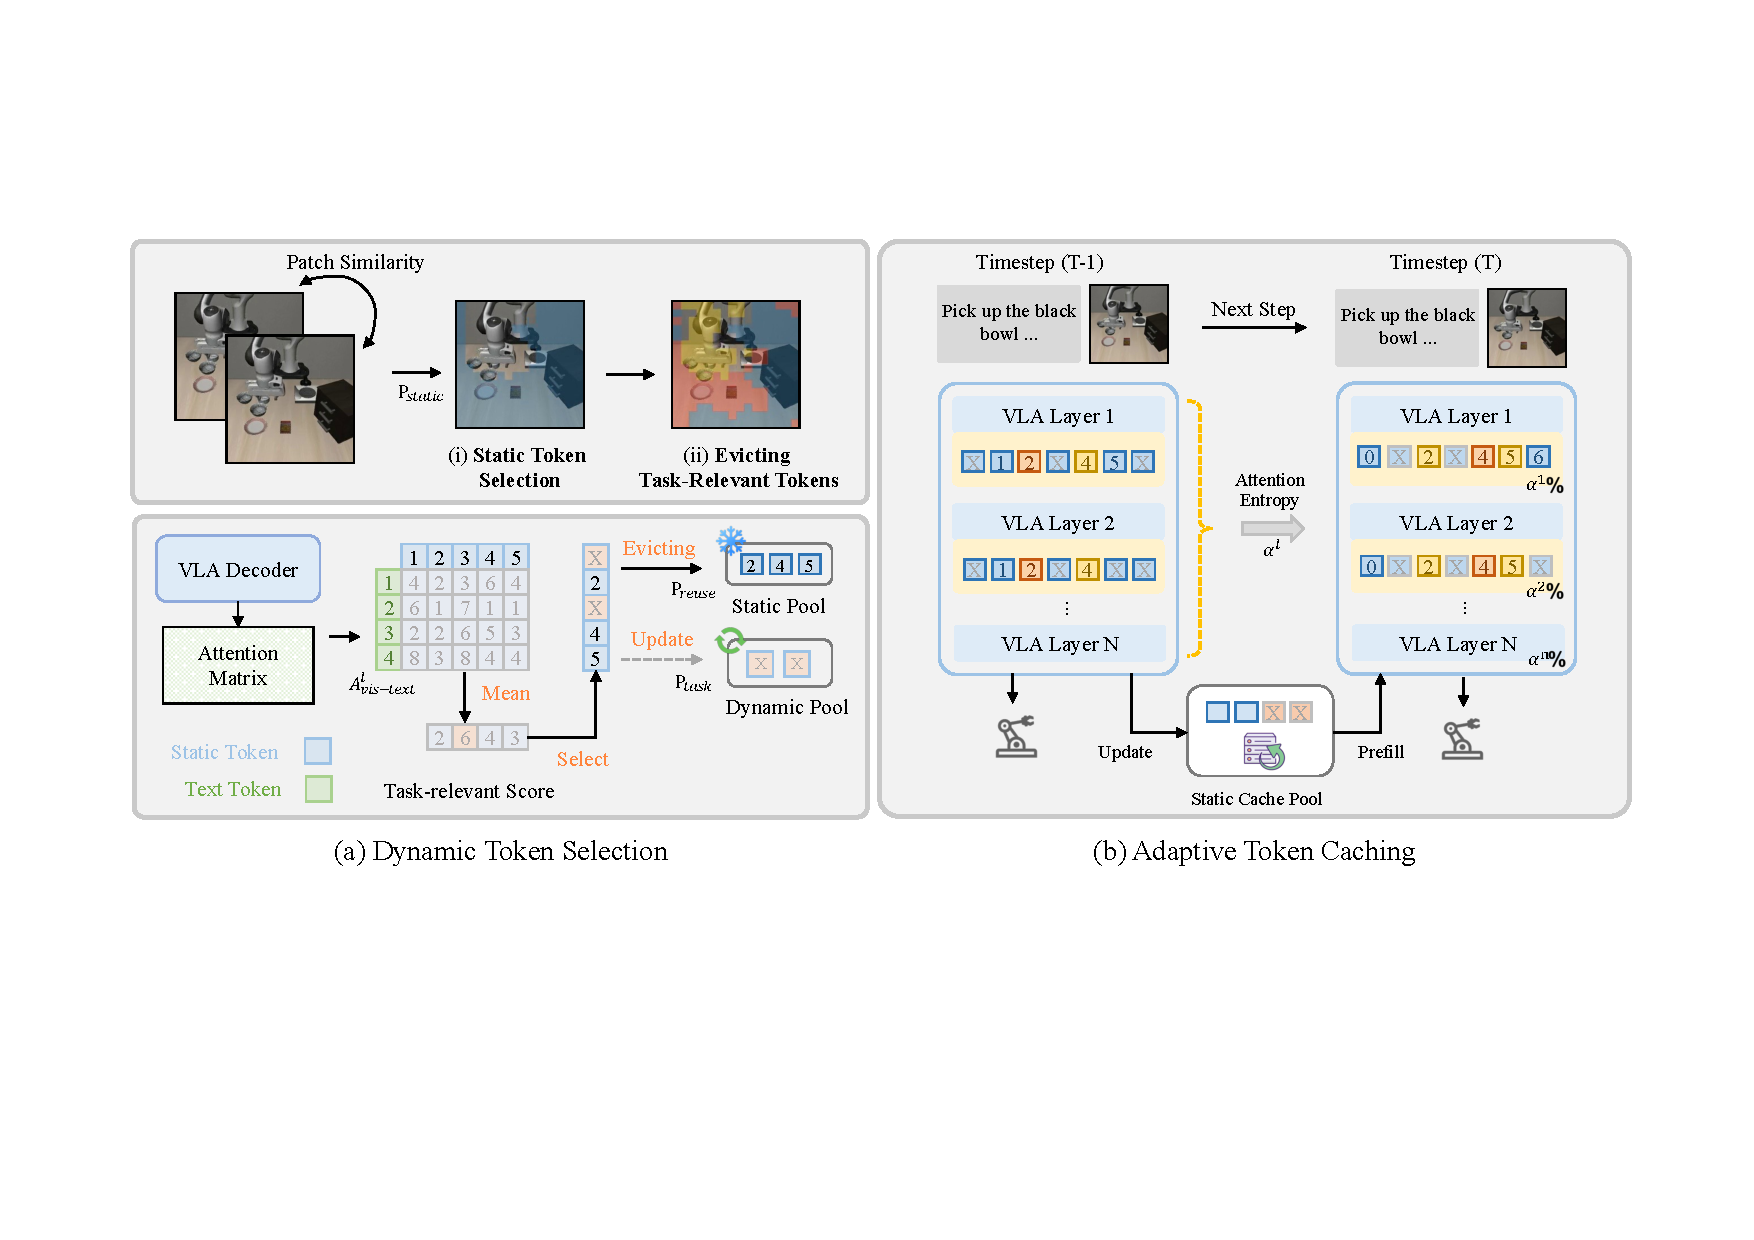
\includegraphics[width=1.0\textwidth]{fig/method.pdf}
% \includegraphics[width=1.0\textwidth]{fig/fig_method1.pdf}
\caption{
\textbf{VLA-Cache} accelerates the VLA's language decoding process across timesteps via the following two steps: (a) \textit{Dynamic Token Selection} reuses static tokens across frames while preserving task-relevant ones; (b) \textit{Adaptive Token Caching} dynamically adjusts reuse ratios per decoder layer based on attention patterns.}
\label{fig:method}
\vspace{-0.6 cm}
\end{figure*}

\subsection{Temporal Redundancy in Robotic Perception}
\label{sec:temporal_redundancy}

In closed-loop robotic manipulation, consecutive visual frames often share large portions of static content. As illustrated in Figure~\ref{fig:method}, background regions and stationary objects typically exhibit negligible changes between adjacent frames. However, most existing Vision-Language-Action (VLA) models discard visual representations after each timestep and recompute all visual tokens from scratch, resulting in substantial redundancy and increased inference latency.

To address this inefficiency, we propose selectively reusing visual tokens that remain static across timesteps. Specifically, we identify and cache the representations of image regions with minimal visual change, allowing their Key-Value (KV) representations to be reused in the next frame. This strategy significantly reduces redundant computation in the VLA visual stream while preserving model performance.

\textbf{Static Token Selection.}
Given an image \(I \in \mathbb{R}^{H \times W \times 3}\), we divide it into \(N \times N\) non-overlapping patches of size \(p \times p\), yielding a set of raw pixel patches \(\mathcal{P}_t = \{ \mathbf{P}_t^{i,j} \}\). For each patch \(\mathbf{P}_t^{i,j}\) in the current frame and its corresponding patch \(\mathbf{P}_{t-1}^{i,j}\) in the previous frame, we compute cosine similarity:
\begin{equation}
\label{eq:sim}
\text{Sim}\big(\mathbf{P}_t^{i,j}, \mathbf{P}_{t-1}^{i,j}\big) 
= \frac{\mathbf{P}_t^{i,j} \cdot \mathbf{P}_{t-1}^{i,j}}{\|\mathbf{P}_t^{i,j}\|_2 \cdot \|\mathbf{P}_{t-1}^{i,j}\|_2}.
\end{equation}

A patch is considered visually static if its similarity exceeds a threshold \(\tau\). We further apply a Top-\(k\) filter to retain the most stable tokens:
\begin{equation}
\label{eq:topk}
\mathcal{P}_{\mathrm{static}} = \mathrm{Top}\text{-}k\Big(\{ \mathbf{P}_t^{i,j} \mid \mathrm{Sim}(\mathbf{P}_t^{i,j}, \mathbf{P}_{t-1}^{i,j}) \ge \tau \}\Big).
\end{equation}

This simple yet effective approach accurately selects truly static tokens across consecutive frames, significantly reducing redundant computations and accelerating inference without compromising overall performance.

\begin{wraptable}{r}{0.45\textwidth}
\centering
\vspace{-0.9cm}
\caption{Comparison of VLA-Cache's core token selection strategies on OpenVLA using the LIBERO Spatial benchmark.}
\small
\setlength{\tabcolsep}{0.5mm}{
\begin{tabular}{lcc}
\toprule
Method & SR (\%) $\uparrow$ & Latency (ms) $\downarrow$ \\
\midrule
OpenVLA & 84.4  & 51.56 \\
+ Static Token        & 74.2  & 31.03 \\
+ Evict Task-Relevant & 82.6  & 31.03 \\
+ Layer Adaptive & 83.8  & 32.22 \\
\bottomrule
\end{tabular}
}
\label{tab:selection_ablation_inline}
\vspace{-0.45cm}
\end{wraptable}
\subsection{Retaining Task-Relevant Information}
\label{sec:task_filtering}

While visual similarity offers a practical signal for reusing static regions, not all visually static tokens are safe to reuse. In robotic control tasks, certain regions, such as the gripper or target object, though visually unchanged, are semantically dynamic and critical for precise action generation. Directly reusing all visually static tokens, without considering their semantic role, can lead to serious performance degradation. As shown in Table~\ref{tab:selection_ablation_inline}, naive static token reuse lowers the success rate from the OpenVLA baseline of \textbf{84.4\%} to just \textbf{74.2\%}. 

This degradation occurs because task-relevant tokens, though minimally changed at the pixel level, exhibit greater feature sensitivity to subtle environmental changes. Unlike vision-language models (VLMs), VLA models must track object states and interactions over time, making them more dependent on accurate visual encoding. Therefore, to ensure alignment with the latest environment state, task-relevant regions must be recomputed each step.


\textbf{Evicting Task-Relevant Tokens.}
To avoid reusing semantically critical but visually static tokens, we propose a lightweight filtering mechanism using cross-attention scores from the language decoder. For each decoder layer \(l\), we extract the text-to-vision attention matrix \(\mathbf{A}^l_{\text{vis-text}}\) from the full attention tensor \(\mathbf{A}^l \in \mathbb{R}^{N_{\text{heads}} \times N_{\text{tokens}} \times N_{\text{tokens}}}\) as:

\begin{equation}
\label{eq:avistext}
\mathbf{A}^l_{\text{vis-text}} 
= \mathbf{A}^l[:,\, v_{\text{start}} : v_{\text{end}},\, t_{\text{start}} : t_{\text{end}}],
\end{equation}
where \( v_{\text{start}}, v_{\text{end}} \) and \( t_{\text{start}}, t_{\text{end}} \) are the indices of the vision and text tokens, respectively. To aggregate the attention scores across multiple heads, we compute the mean attention for each vision token as $\mathbf{A}^l_{\text{avg}} 
= \mathrm{Mean}_{\text{heads}}\!\bigl(\mathbf{A}^l_{\text{vis-text}}\bigr)$. For task relevance across multiple layers \( \mathcal{L} \), the final task relevance scores are obtained by averaging the scores across the selected layers as $\mathbf{S}_{\text{task-relevance}} 
= \mathrm{Mean}_{l \in \mathcal{L}}\!\bigl(\mathbf{A}^l_{\text{avg}}\bigr)$.
Using these scores, we rank the vision tokens based on their task relevance and apply a threshold \( \tau_{\text{task}} \) to select the most task-relevant tokens:
\begin{equation}
\label{eq:ptask}
\mathcal{P}_{\text{task-relevant}} 
= \{ \mathbf{P}_t^{i,j} \mid \mathbf{S}_{\text{task-relevance}}[i,j] \geq \tau_{\text{task}} \}.
\end{equation}

Finally, we combine the set of static tokens \( \mathcal{P}_{\mathrm{static}} \) selected in the first step with the task-relevant tokens. Tokens that are both static and highly task-relevant are removed from the reusable token set to ensure they are recomputed in the current step:
\begin{equation}
\label{eq:pfinal}
\mathcal{P}_{\mathrm{reuse}} 
= \mathcal{P}_{\mathrm{static}} \;\setminus\; \mathcal{P}_{\text{task-relevant}}.
\end{equation}
By filtering out semantically significant tokens from the static reuse set, our method restores the degraded success rate from \textbf{74.2\%} to \textbf{82.6\%}, while maintaining the computational gains in FLOPs and latency. This balance between task fidelity and efficiency illustrates the value of cross-modal attention as a lightweight signal for safe token reuse in VLA models.


\begin{figure}[t]
\centering
% Insert both algorithms side-by-side
\begin{minipage}{0.48\textwidth}
\begin{algorithm}[H]
\caption{Dynamic Token Selection}
\label{alg:dynamic_token_selection}
\begin{algorithmic}[1]
\STATE \textbf{Input:} Frames $\{I_{t-1}, I_t\}$, thresholds $\tau$, $\tau_{\text{task}}$, hyperparameter $k$
\STATE \textbf{Output:} Reusable token indices $\mathcal{P}_{\mathrm{final}}$

\STATE \textcolor{mygreen}{\COMMENT{\textit{Static Token Selection}}}
\STATE Patchify both frames $I_{t-1}, I_t$ and compute $\text{Sim}(\mathbf{P}_t, \mathbf{P}_{t-1})$ among related patches
\STATE Select $\mathcal{P}_{\text{static}}$ where similarity $\geq \tau$
\STATE Apply top-$k$ filtering to refine static token selection
\STATE \textcolor{mygreen}{\COMMENT{\textit{Evict Task-Relevant Tokens}}}
\STATE Compute text-to-vision attention scores $\mathbf{S}_{\text{task-relevance}}$
\STATE Select $\mathcal{P}_{\text{task-relevant}}$ where attention $\geq \tau_{\text{task}}$
\STATE Compute reusable tokens: $\mathcal{P}_{\mathrm{final}} = \mathcal{P}_{\text{static}} \setminus \mathcal{P}_{\text{task-relevant}}$

\STATE \textbf{return} $\mathcal{P}_{\mathrm{final}}$
\end{algorithmic}
\vskip 0.04in
\end{algorithm}
\end{minipage}
\hfill
\begin{minipage}{0.48\textwidth}
\begin{algorithm}[H]
\caption{Adaptive Token Caching}
\label{alg:adaptive_token_caching}
\begin{algorithmic}[1]
\STATE \textbf{Input:} Token indices $\mathcal{P}_{\mathrm{final}}$, previous KV cache $\{\mathbf{K}_{t-1}^l, \mathbf{V}_{t-1}^l\}$, representations $\mathbf{H}_t^l$
\STATE \textbf{Output:} Updated KV cache $\{\mathbf{K}_t^l, \mathbf{V}_t^l\}$

\STATE Compute entropy $R_{\text{cum}}^l$, reuse ratio $\alpha^l$, subset $\mathcal{P}_{\mathrm{reuse}} \subseteq \mathcal{P}_{\mathrm{final}}$

\FOR{each layer $l$ and token $i$}
    \IF{$i \in \mathcal{P}_{\mathrm{reuse}}$} 
    \STATE Reuse cached values: \\
           $\mathbf{K}_t^l(i) = \mathbf{K}_{t-1}^l(i), \mathbf{V}_t^l(i) = \mathbf{V}_{t-1}^l(i)$
    \ELSE
    \STATE Recompute:\\$\mathbf{K}_t^l(i) = W_K^l \mathbf{H}_t^l(i)$, \\ $\mathbf{V}_t^l(i) = W_V^l \mathbf{H}_t^l(i)$
    \ENDIF
\ENDFOR
\STATE \textbf{return} $\{\mathbf{K}_t^l, \mathbf{V}_t^l\}$
\end{algorithmic}
\vskip -0.02in
\end{algorithm}
\end{minipage}
\label{fig:dual_algorithm}
\vskip -0.2in
\end{figure}

\subsection{Layer Adaptive Token Reusing}
While static token selection and task-relevance filtering eliminate a large portion of redundant computation, we observe that attention distributions within the VLA decoder vary significantly across different layers. This finding is consistent with observations reported by prior work \textit{FastV}~\cite{chen2025image}, indicating that both VLA and VLM decoders exhibit similar patterns of attention flow: early layers display dispersed attention, followed by fluctuations in intermediate layers, and eventually a partial rebound near the final layers.

To account for these differences, we propose a \textit{layer-adaptive strategy} that adjusts the fraction of reused tokens based on each layer’s attention concentration. Specifically, we quantify the attention distribution at layer \(l\) via an \emph{entropy} measure, following the same mean-attention computation described in Eq. ~\ref{eq:avistext}. Let \(\mathcal{E}^l\) denote the resulting entropy. We then define an \emph{entropy ratio} \(R^l=(\mathcal{E}^{l-1} - \mathcal{E}^l)/\mathcal{E}^{l-1}\), which captures how much more concentrated the attention is in layer \(l\) compared to layer \(l-1\).

A positive $R^l$ indicates that the attention distribution at layer $l$ is more focused than that of layer $l-1$. We accumulate these ratios across layers to obtain a cumulative score, which in turn determines the proportion \(\alpha^l\) of static tokens (from \(\mathcal{P}_{\mathrm{final}}\)) that are reused at layer \(l\). Formally,
\begin{equation}
\label{eq:reuse_ratio}
\alpha^l \;=\; \min\Bigl(k \sum_{j=1}^l R^j,\; 1\Bigr),
\end{equation}
where \(k\) is a hyperparameter that governs the impact of attention concentration. Layers with larger cumulative entropy reduction are allowed to reuse a higher fraction of tokens, reflecting the insight that as attention becomes more focused, fewer tokens are likely to require recomputation.

In practice, this layer-adaptive mechanism dynamically adjusts token reuse based on the evolving attention patterns in the VLA decoder, effectively balancing computational efficiency with task accuracy. By selectively retaining only the most relevant tokens at each layer, our method significantly reduces redundant computations while maintaining reliable action prediction. 

\section{Implementations}

\subsection{Cross-Frame Visual Token Caching}
During inference, VLA-Cache accelerates robotic action prediction by reusing previously computed key-value (KV) representations of visual tokens across time. Instead of recomputing all visual tokens in each time step, the model identifies a subset of static tokens, those that exhibit minimal change across frames, and reuses their cached representations from the previous time step. In contrast, dynamic tokens, which undergo significant visual change or are task-relevant, are freshly computed to maintain accurate action generation.

At each timestep $t$, given the visual token sequence $\mathbf{H}_t$, the model identifies a subset $\mathcal{P}_{\text{reuse}}$ of tokens that remain unchanged from the previous frame and reuses their cached representations:
\begin{equation}
\mathbf{K}_t(i) =
\begin{cases}
\mathbf{K}_{t-1}(i), & i \in \mathcal{P}_{\text{reuse}} \\
W_K \mathbf{H}_t(i), & \text{otherwise}
\end{cases}, \quad
\mathbf{V}_t(i) =
\begin{cases}
\mathbf{V}_{t-1}(i), & i \in \mathcal{P}_{\text{reuse}} \\
W_V \mathbf{H}_t(i), & \text{otherwise}
\end{cases}.
\end{equation}
This design avoids redundant computation for static tokens while ensuring dynamic or task-relevant inputs are freshly computed. Most existing approaches reduce computation by pruning or merging tokens within a single frame~\cite{chen2025image, zhang2024sparsevlm, bolya2022token, cao2023pumer, cao2024madtp}. In contrast, VLA-Cache exploits temporal redundancy by caching and reusing visual tokens across frames, making it better aligned with the closed-loop nature of robotic control. Notably, it is compatible with high-frequency architectures and directly alleviates the \textit{decoding bottleneck}. Since it requires no model modification or retraining, VLA-Cache serves as a \textit{plug-and-play} optimization for efficient robotic inference.
An overview of the inference procedure is shown in Algorithm~\ref{alg:dynamic_token_selection} and Algorithm~\ref{alg:adaptive_token_caching}, detailing token selection and adaptive caching. Additional implementation details are provided in Appendix~\ref{app:inference_detail}.


\subsection{Theoretical Analysis of Computational Complexity}
\label{method:Computational_Complexity}
\noindent
\textbf{Overhead of Token Selection.} 
The cost of static token identification is approximately $\mathcal{O}(H^2)$ due to patch similarity checks, while task-relevance filtering introduces a cross-modal attention aggregation cost of $\mathcal{O}(L_t L_v D)$. The entropy-based layer-adaptive strategy incurs an additional $\mathcal{O}(L^2 D)$ complexity, which remains significantly lower than the baseline per-layer cost.

\noindent
\textbf{Computational Cost Reduction.} 
In standard VLA inference, each Transformer layer processes $L$ tokens, with a total FLOP cost per layer:
\begin{equation}
\label{eq:baseline_layer_flops}
\text{FLOPs} \approx 4 L D^2 + 2 L^2 D + 2 L D M.
\end{equation}
VLA-Cache reduces effective token count per layer to $L_r = \alpha \times \mathcal{P}_{\mathrm{final}}$, leading to theoretical savings:
\begin{equation}
\label{eq:reuse_saving}
\Delta \text{FLOPs}_{\mathrm{layer}} \approx 4 L_r D^2 + 2 L_r^2 D + 2 L_r D M.
\end{equation}


\noindent
\textbf{Total Complexity Reduction.} 
Bringing all components together, the theoretical overall FLOP reduction per layer is:
\begin{equation}
\label{eq:final_theoretical_gain}
\begin{aligned}
\Delta \text{FLOPs}_{\text{total}} 
\approx  \Bigl( 4 L_r D^2 + 2 L_r^2 D + 2 L_r D M \Bigr) - \Bigl( H^2 + L_t L_v D + L^2 D \Bigr).
\end{aligned}
\end{equation}

Please refer to Appendix~\ref{appendix:complexity} for detailed derivations, including static token selection costs, attention filtering complexity, and layer-adaptive entropy calculations.

